%% =====================================================================
\section{Design and Implementation of CacheCollapse}
\label{sec:design}
%% =====================================================================

\subsection{Design Goals}
The testbed was designed around five requirements: (R1)~\emph{fidelity}---use the same
industry-standard components and request path as a production service;
(R2)~\emph{isolation}---never send attack traffic outside a private network;
(R3)~\emph{controllability}---switch traffic, attack, and each defense independently
and live; (R4)~\emph{observability}---measure every quantity needed for detection and
evaluation at sub-second resolution; and (R5)~\emph{reproducibility}---bring the entire
system up, or reset it, with one command.

\subsection{Architecture Overview}
CacheCollapse is a nine-service Docker Compose application on a single isolated bridge
network (Figure~\ref{fig:arch}, Table~\ref{tab:services}). Each service runs in its
own container, so that resource use can be attributed per component and the system
can be reset between runs. The public request path is
Nginx~$\rightarrow$~Flask~$\rightarrow$~Redis, with PostgreSQL read only on a cache
miss. Redis additionally serves as a lightweight \emph{control bus}: the dashboard
writes run-state and defense flags that the load generator and the Flask application
read on every iteration or request, so every experiment can be driven from a browser.

\begin{figure}[t]
\centering
\resizebox{\linewidth}{!}{%
\begin{tikzpicture}[
  font=\small,
  box/.style={draw, rounded corners=2pt, minimum width=2.45cm, minimum height=0.95cm, align=center, fill=white},
  core/.style={box, fill=blue!6},
  mon/.style={box, fill=green!6},
  ext/.style={box, fill=orange!8},
  arr/.style={-{Stealth[length=2.2mm]}, thick},
  dash/.style={-{Stealth[length=2mm]}, densely dashed}]
\node[ext]  (lg) at (0,1.4)    {Load generator\\\footnotesize normal + burst};
\node[ext]  (br) at (0,-1.6)   {Browser\\\footnotesize dashboard / shop};
\node[core] (ng) at (3.5,0)    {Nginx\\\footnotesize proxy + edge RL};
\node[core] (fl) at (7.0,0)    {Flask app\\\footnotesize lock + SWR + app RL};
\node[core] (rd) at (10.6,1.4) {Redis\\\footnotesize cache + control bus};
\node[core] (pg) at (10.6,-1.4){PostgreSQL\\\footnotesize victim DB};
\node[mon]  (fe) at (3.5,-3.3) {Frontend\\\footnotesize static UI};
\node[mon]  (mo) at (7.0,-3.3) {Monitor\\\footnotesize rule + ML, CSV, SSE};
\node[mon]  (pr) at (10.6,-3.6){Prometheus};
\node[mon]  (gr) at (13.8,-3.6){Grafana};
\draw[arr] (lg) -- (ng);
\draw[arr] (br) -- (ng);
\draw[arr] (ng) -- node[above,font=\footnotesize]{/api} (fl);
\draw[arr] (fl) -- node[above,sloped,font=\footnotesize]{get/set} (rd);
\draw[arr] (fl) -- node[below,sloped,font=\footnotesize]{on miss} (pg);
\draw[dash] (ng) -- node[left,font=\footnotesize]{/} (fe);
\draw[dash] (ng) -- node[above,sloped,font=\footnotesize]{/live, /control} (mo);
\draw[dash] (mo) -- node[right,font=\footnotesize,pos=0.4]{scrape /metrics} (fl);
\draw[dash] (pr.north west) -- node[above,sloped,font=\footnotesize]{scrape} (fl.south east);
\draw[arr] (pr) -- (gr);
\draw[dash] (mo.east) -| node[right,font=\footnotesize,pos=0.75]{flags} (8.75,1.4) -- (rd.west);
\begin{scope}[on background layer]
\node[draw=black!30, dashed, rounded corners, inner sep=8pt, fit=(ng)(fl)(rd)(pg)(mo)(fe)(pr)(gr)] (net) {};
\node[anchor=north east, font=\footnotesize, black!60] at (net.north east) {private Docker bridge network \texttt{cachenet}};
\end{scope}
\end{tikzpicture}}
\caption{CacheCollapse architecture. Solid arrows: request path; dashed arrows: control
and observation paths. ``RL'' denotes rate limiting and ``SWR'' stale-while-revalidate.
The load generator is drawn outside for clarity but is itself a container attached to
the same network, so that attack traffic never leaves the host; the browser reaches the
stack through the published proxy port.}
\label{fig:arch}
\end{figure}

\begin{table}[t]
\centering
\caption{CacheCollapse containerized services (images and versions as deployed).}
\label{tab:services}
\small
\begin{tabularx}{\linewidth}{@{}cL{2.0cm}L{3.3cm}Y@{}}
\toprule
\# & Service & Image / runtime & Role \\
\midrule
1 & Nginx & \texttt{nginx:1.27-alpine} & Public reverse proxy (port 8090); routing; edge \texttt{limit\_req}; live reload watcher \\
2 & Flask app & Python 3.12, Flask 3.0.3, Gunicorn 22 (1 worker, 200 threads) & \texttt{GET /products/<id>}; cache locking, stale-while-revalidate, app rate limiting; \texttt{/metrics} \\
3 & Redis & \texttt{redis:7-alpine} & Product cache (TTL 4~s), stale copies, locks, rate-limit counters, control bus \\
4 & PostgreSQL & \texttt{postgres:16-alpine} & Victim database; 100 seeded products; health-checked \\
5 & Load generator & Python 3.12, aiohttp 3.10.5 & Asynchronous normal traffic and burst attack, driven by Redis flags \\
6 & Monitor & Python 3.12, Flask, scikit-learn 1.5.1 & 2~Hz metric collection, rule + ML detection, CSV log, SSE feed, control API \\
7 & Frontend & \texttt{nginx:1.27-alpine} (static) & Live dashboard (Chart.js 4.4.1 \cite{chartjs}) and ``CacheShop'' storefront \\
8 & Prometheus & \texttt{prom/prometheus:v2.54.1} & Scrapes backend every 2~s \\
9 & Grafana & \texttt{grafana/grafana:11.2.0} & Provisioned dashboard over Prometheus \\
\bottomrule
\end{tabularx}
\end{table}

\subsection{Data Model and Seed Data}
The database holds a single \texttt{products} table (\texttt{id}, \texttt{name},
\texttt{description}, \texttt{price}, \texttt{stock}, \texttt{updated\_at}) seeded with
100 synthetic records at first start; no real data is used anywhere in the system. To
make database cost visible at laboratory scale, each product read executes
\texttt{pg\_sleep($d_0$)} alongside the \texttt{SELECT}, with $d_0=110$~ms
(configurable via \texttt{DB\_QUERY\_DELAY\_MS}). This models an expensive query---a
join, an aggregation, or a cold page read---without requiring a large dataset, and it
holds a pooled connection for the duration, which is exactly the resource the attack
exhausts. The connection pool is a psycopg2 \texttt{ThreadedConnectionPool} with
$c_{\min}=2$ and $c=12$ connections; when all are in use, the next request fails
immediately and the application returns HTTP~503.

\subsection{Concurrency Model}
The application runs under Gunicorn with a single worker process and 200 threads.
Two considerations drove this choice. First, a stampede requires real concurrency at
the application tier, so that many requests can be between ``cache miss'' and
``database query'' at the same time. Second, Prometheus client counters live in
process memory; with several worker processes each would hold a separate copy and the
monitor would observe only one of them. A single multi-threaded worker keeps counters
consistent while still admitting hundreds of concurrent requests. Nginx uses
\texttt{worker\_processes auto} and 8{,}192 connections per worker so that the proxy is
not the first bottleneck, and keeps 64 upstream keep-alive connections to the
application.

\subsection{The Read Path and Mitigation I: Cache Locking with Stale-While-Revalidate}
\label{sec:design-lock}
Algorithm~\ref{alg:read} gives the read path. On a hit, the cached JSON is returned.
On a miss with locking disabled, the request queries the database directly---this is
the vulnerable stampede path. With locking enabled, the request attempts to acquire a
per-key mutex in Redis with \texttt{SET lock:<key> 1 NX PX 3000}, an atomic
set-if-absent with a 3~s expiry \cite{redisdocs}. The single winner queries the
database and writes two copies of the result: a \emph{fresh} copy under the normal TTL
($T=4$~s) and a \emph{stale} copy under a much longer TTL ($15T=60$~s). Every other
concurrent miss---a ``loser''---immediately returns the stale copy instead of waiting.
Thus $N$ simultaneous misses produce exactly one database query, and losers are served
in cache time rather than regeneration time. Only if no stale copy exists does a loser
poll the fresh key every 50~ms for up to 1.5~s before falling back to the database.

To remove that cold-start window, the application \emph{pre-warms} a stale copy of
every product (with a one-hour TTL) at start-up, using a single fast query without the
artificial delay. The fresh cache is deliberately \emph{not} pre-warmed, so that the
attack still produces genuine misses. This is the security-oriented generalization of
memcache leases \cite{nishtala2013} and of the stale-serving stability pattern
\cite{nygard2018,rfc5861}.

\begin{algorithm}[t]
\caption{Product read path with single-flight locking and stale-while-revalidate}
\label{alg:read}
\begin{algorithmic}[1]
\Function{LoadProduct}{$id$}
  \State $k \gets \texttt{"product:"}\,id$; \quad $s \gets \texttt{"stale:"}\,k$
  \If{$v \gets \Call{Get}{k}$ exists} \State \textsc{CountHit}; \Return $v$ \EndIf
  \State \textsc{CountMiss}
  \If{\textbf{not} \Call{Flag}{cache\_lock}} \State \Return \Call{QueryAndFill}{$k,s,id$} \Comment{vulnerable path}\EndIf
  \If{\Call{SetNX}{\texttt{"lock:"}$k$, ttl$=3$\,s}} \Comment{lock winner}
     \State \textbf{try} \Return \Call{QueryAndFill}{$k,s,id$} \textbf{finally} \Call{Del}{\texttt{"lock:"}$k$}
  \EndIf
  \If{$v \gets \Call{Get}{s}$ exists} \State \textsc{CountHit}; \Return $v$ \Comment{serve stale, no wait}\EndIf
  \For{$i \gets 1$ \textbf{to} 30} \Comment{cold start only: poll 50 ms, up to 1.5 s}
     \State \Call{Sleep}{50 ms}
     \If{$v \gets \Call{Get}{k}$ exists} \State \textsc{CountHit}; \Return $v$ \EndIf
  \EndFor
  \State \Return \Call{QueryAndFill}{$k,s,id$}
\EndFunction
\Statex
\Function{QueryAndFill}{$k,s,id$}
  \State \textsc{CountDbQuery}
  \State $v \gets$ \Call{DbGetProduct}{$id$} \Comment{raises PoolBusy $\Rightarrow$ HTTP 503}
  \State \Call{Set}{$k, v$, ttl$=T$}; \Call{Set}{$s, v$, ttl$=15T$}
  \State \Return $v$
\EndFunction
\end{algorithmic}
\end{algorithm}

\paragraph{Correctness notes.} Three properties of this implementation deserve comment.
(i)~The database query counter is incremented \emph{before} a pool connection is
obtained, so the metric counts query \emph{attempts}, including those rejected because
the pool is exhausted (Section~\ref{sec:mechanics}). (ii)~A loser served from the stale
copy increments both the miss and the hit counter, so under defense the hit and miss
counts overlap and the computed miss ratio is biased downward. (iii)~The lock is
released with an unconditional \texttt{DEL}. If a winner ever held the lock longer than
its 3~s expiry, it could delete a lock acquired by a later winner. With a 110~ms query
this does not occur in practice, but a production implementation should store a unique
token and release with an atomic compare-and-delete, and should not rely on the lock
for correctness of writes \cite{kleppmann2016}.

\subsection{Mitigation II: Layered Rate Limiting}
\label{sec:design-rl}
Rate limiting sheds the attacker's excess concurrency at two layers.

\paragraph{Application layer.} Inside Flask, a fixed-window per-client limiter
(Listing~\ref{lst:applimit}) increments a Redis counter keyed by client and current
second and rejects requests beyond $R=50$ per second with HTTP~429
\cite{rfc6585}. Because it reads its on/off flag from Redis on every request, it can be
toggled live without a restart. The client identity is taken from the
\texttt{X-Forwarded-For} header, which Nginx \emph{overwrites} with the real peer
address (\texttt{proxy\_set\_header X-Forwarded-For \$remote\_addr}), so a client cannot
evade the limiter by supplying its own header. An earlier version omitted this header;
the limiter then saw every request as coming from the proxy, and the attacker consumed
the shared budget of legitimate users (Section~\ref{sec:lessons}).

\begin{lstlisting}[language=Python, caption={Application-layer fixed-window limiter (\texttt{backend/app.py}).}, label={lst:applimit}]
def rate_limited(client):
    bucket = "rl:%s:%d" % (client, int(time.time()))
    n = r.incr(bucket)            # atomic in Redis
    if n == 1:
        r.expire(bucket, 2)       # window garbage-collects itself
    return n > RATE_LIMIT_RPS     # 50 req/s per client
\end{lstlisting}

\paragraph{Edge layer.} Nginx defines a leaky-bucket zone keyed on the binary client
address at 50~req/s (\texttt{limit\_req\_zone \$binary\_remote\_addr zone=api\_rl:10m
rate=50r/s}). Whether the zone is \emph{applied} is controlled by a one-line include
file inside the \texttt{/api/} location. When an operator enables rate limiting, the
monitor rewrites that file to \texttt{limit\_req zone=api\_rl burst=20 nodelay;}; a
watcher loop in the Nginx container compares the file with its previous contents every
second and runs \texttt{nginx -s reload} on change. Excess requests are then rejected
at the proxy, before they consume an upstream connection, an application thread, or a
pool slot. Note that, unless configured otherwise with \texttt{limit\_req\_status},
Nginx rejects with HTTP~503; these rejections never reach the application and are
therefore \emph{not} counted as application failures in our metrics, but a client sees
them as 503s. We recommend \texttt{limit\_req\_status 429} in production so that
intentional shedding is distinguishable from overload at the client as well.

\subsection{Control Plane}
\label{sec:control}
All live state is held in Redis (Table~\ref{tab:controlkeys}). The dashboard calls the
monitor's control API (\texttt{POST /control/\{traffic, attack, defense, preset,
reset\}}); the monitor sets the corresponding keys; the load generator polls
\texttt{run:*} keys every 100--200~ms and the application reads \texttt{cfg:*} keys on
every request. The \emph{reset} action clears fresh cache entries, locks, and
rate-limit buckets so that the next experiment starts with a cold cache, but
deliberately keeps the stale safety net. Three \emph{presets} configure the three
experimental conditions in one click.

\begin{table}[t]
\centering
\caption{Redis key space used by CacheCollapse.}
\label{tab:controlkeys}
\small
\begin{tabularx}{\linewidth}{@{}L{3.4cm}L{2.6cm}Y@{}}
\toprule
Key pattern & Writer / reader & Purpose \\
\midrule
\texttt{product:<id>} & app / app & Fresh cached product (TTL 4~s) \\
\texttt{stale:product:<id>} & app / app & Stale copy for SWR (TTL 60~s; 3{,}600~s when pre-warmed) \\
\texttt{lock:product:<id>} & app / app & Single-flight mutex (\texttt{NX PX 3000}) \\
\texttt{rl:<client>:<second>} & app / app & Fixed-window rate-limit counter (expires after 2~s) \\
\texttt{run:traffic}, \texttt{run:attack} & monitor / load gen. & Start/stop normal traffic and attack \\
\texttt{cfg:cache\_lock}, \texttt{cfg:rate\_limit} & monitor / app & Toggle defenses live \\
\bottomrule
\end{tabularx}
\end{table}

\subsection{Traffic Generation}
\label{sec:design-loadgen}
A single asynchronous generator (aiohttp) runs two independent loops that target the
public proxy, exactly as an external client would. The \emph{normal} loop issues
batches of four concurrent requests for uniformly random products (ids 1--100) and
sleeps 100~ms between batches, which yields ${\approx}17$--$18$~req/s
(Section~\ref{sec:model}). The \emph{attack} loop issues bursts of $B=250$ concurrent
requests for a single product, rotating through a pool of $H=20$ hot products (ids
1--20) with a 50~ms pause between bursts. Rotation converts an isolated one-shot
stampede into a sustained overload: each hot key is revisited only after all others,
by which time its entry has expired. Starting the attack also starts normal traffic, so
the attack is always superimposed on a normal background. The generator's connection
pool allows $B+100$ concurrent connections and a 15~s total timeout per request.

\subsection{Instrumentation and the Monitor}
\label{sec:design-monitor}
The application exposes Prometheus metrics (Table~\ref{tab:metrics}). The monitor
scrapes them every $\Delta=0.5$~s, differences consecutive cumulative snapshots, and
computes per-interval quantities:
\begin{align}
\text{rps} &= \frac{\Delta n_{\mathrm{req}}}{\Delta t}, \quad
q_{db} = \frac{\Delta n_{\mathrm{db}}}{\Delta t}, \quad
m = \frac{\Delta n_{\mathrm{miss}}}{\Delta n_{\mathrm{hit}} + \Delta n_{\mathrm{miss}}}, \quad
\bar{L} = \frac{\Delta \Sigma_{\mathrm{lat}}}{\Delta n_{\mathrm{lat}}},
\label{eq:rates}
\end{align}
where $\Delta t$ is the measured time between scrapes. The 95th-percentile latency is
approximated from the change in histogram buckets: the smallest bucket upper bound at
which the cumulative count reaches 95\% of the interval's observations. Because the
histogram has bounds $\{10, 50, 100, 250, 500, 1000, 2000, 5000, 10000\}$~ms, this p95
is quantized to those values. Failures are recorded as the \emph{count} of HTTP~503
responses in the interval; we convert to a rate by dividing by $\Delta t$ in all
analyses (Section~\ref{sec:validity}).

\begin{table}[t]
\centering
\caption{Prometheus metrics exported by the application.}
\label{tab:metrics}
\small
\begin{tabularx}{\linewidth}{@{}L{4.2cm}L{2.0cm}Y@{}}
\toprule
Metric & Type & Meaning \\
\midrule
\texttt{cc\_requests\_total\{result\}} & counter & Requests by outcome: ok, not\_found, overloaded, rate\_limited \\
\texttt{cc\_db\_queries\_total} & counter & Database query \emph{attempts} \\
\texttt{cc\_cache\_hits\_total} & counter & Cache hits (fresh, or stale served to a lock loser) \\
\texttt{cc\_cache\_misses\_total} & counter & Fresh-cache misses \\
\texttt{cc\_failed\_total} & counter & HTTP 503: pool exhausted (genuine overload) \\
\texttt{cc\_rejected\_total} & counter & HTTP 429: shed by the app limiter (defense working) \\
\texttt{cc\_latency\_seconds} & histogram & Request latency inside the application \\
\bottomrule
\end{tabularx}
\end{table}

The monitor derives the system \emph{mode} from the control flags (idle, normal,
attack, or protected---the last meaning ``attack running with at least one defense
enabled'') and a \emph{health} predicate,
\begin{equation}
\mathrm{healthy} \iff q_{db} < 2\max(\bar q_{\mathrm{base}},5)\ \wedge\ \bar L < 120~\text{ms}\ \wedge\ n_{503} < 3,
\label{eq:healthy}
\end{equation}
from which it reports a status (healthy, overloaded, protected, or degraded). It also
records, per attack, the \emph{detect time} (attack start to first alert) and the
\emph{recover time} (first unhealthy interval to the next healthy one). Each interval
is appended to a CSV file with the columns listed in Table~\ref{tab:csv}
(Section~\ref{sec:method}) and pushed to the dashboard via SSE.

\subsection{Detection I: Multi-Signal Rule}
\label{sec:design-rule}
The rule encodes the stampede's signature: database load, latency, and cache-miss rate
must be elevated \emph{at the same time},
\begin{equation}
\mathrm{alert}_{\mathrm{rule}} \iff
\big(q_{db} > K\cdot\max(\bar{q}_{\mathrm{base}}, 5)\big) \wedge
\big(\bar{L} > \tau_L\big) \wedge
\big(m > \tau_m\big),
\label{eq:rule}
\end{equation}
with $K=5$, $\tau_L=200$~ms, and $\tau_m=0.5$. The baseline $\bar{q}_{\mathrm{base}}$
is an exponentially weighted moving average,
$\bar q \leftarrow 0.8\,\bar q + 0.2\,q_{db}$, updated only during steady normal
traffic; the floor of 5~queries/s prevents a near-zero baseline from making the first
condition trivially true. The rationale is that a benign flash crowd raises request
volume but is served from cache, so it does not simultaneously raise database load.
For the first $W=6$ intervals (3~s) after normal traffic starts, all alerts are
suppressed: the cache is cold, every request misses, and the start-up transient would
otherwise look exactly like an attack. Because the rule's alert names which conditions
held, it is fully explainable on the dashboard.

\subsection{Detection II: Unsupervised IsolationForest}
\label{sec:design-ml}
The ML detector (Algorithm~\ref{alg:ml}) is an IsolationForest \cite{liu2008} trained
only on normal traffic, with no attack samples and no labels. Each interval yields a
feature vector $\mathbf{x}=[\,q_{db}, \bar{L}, m, \text{rps}, n_{503}\,]$. Features
are standardized to zero mean and unit variance with statistics from the baseline
window, so that every signal contributes on a comparable scale. The model is first
fitted once ten baseline samples (5~s) are available and is refitted on every new
baseline sample over a sliding window of at most 300 samples. Scikit-learn defaults
are used for the forest (100 trees, sub-sample size $\min(256,n)$), with
\texttt{contamination}$=0.01$ and a fixed random seed. An interval is anomalous if the
forest's \texttt{predict} returns $-1$; an alert requires two consecutive anomalous
intervals (debounce), which removes single-interval blips while delaying a sustained
attack by at most one interval. A normalized score
$\tilde s = \mathrm{clip}(0.5 - 4\,\mathrm{decision\_function}(\mathbf{x}), 0, 1)$ drives
the dashboard gauge only.

\begin{algorithm}[t]
\caption{Online IsolationForest detector}
\label{alg:ml}
\begin{algorithmic}[1]
\State $\mathcal{B} \gets [\,]$; model $\gets$ \textsc{None}; $h \gets 0$
\For{each interval with features $\mathbf{x}$ and mode $\mu$}
  \If{$\mu=$ normal \textbf{and} warm-up passed \textbf{and} $q_{db}>0$}
    \State append $\mathbf{x}$ to $\mathcal{B}$; keep last 300
    \If{$|\mathcal{B}|\ge 10$} \State scaler $\gets$ \textsc{StandardScaler}.fit($\mathcal{B}$); model $\gets$ \textsc{IForest}(cont.$=0.01$).fit(scaler($\mathcal{B}$)) \EndIf
  \EndIf
  \If{model $=$ \textsc{None}} \State anomalous $\gets$ \textbf{false}
  \Else \State anomalous $\gets$ model.predict(scaler($\mathbf{x}$)) $= -1$ \EndIf
  \If{$\mu=$ normal \textbf{and} within warm-up} \State anomalous $\gets$ \textbf{false} \EndIf
  \State $h \gets h+1$ \textbf{if} anomalous \textbf{else} $0$
  \State $\mathrm{alert}_{\mathrm{ML}} \gets (h \ge 2)$
\EndFor
\end{algorithmic}
\end{algorithm}

\subsection{User Interfaces}
\label{sec:ui}
The \emph{live operations console} (Figure~\ref{fig:ui}) is a single static page that
subscribes to the monitor's SSE feed and renders, at 2~Hz, a status pill, a detection
banner, six key-number tiles (requests/s, cache hit rate, database queries/s, failed
requests, detect time, recover time), four live charts (response time, database
queries/s, cache hits vs.\ misses, ok vs.\ failed requests), and two detector panels
(the rule's three condition lamps and the ML anomaly gauge). A left rail holds the
traffic controls, the two defense toggles, and the three experiment presets. A
separate \emph{CacheShop} storefront loads twelve hot products every refresh and
shows each item's load time, giving a customer's-eye view of availability. Each fetch
has a 4~s timeout (\texttt{AbortController}) and the next refresh is scheduled only
after the current one completes, a fix for a bug in which hung requests piled up and
left the page stuck after an attack (Section~\ref{sec:lessons}). Grafana provides a
second, industry-standard view with four provisioned panels (database queries/s,
average latency, cache hits vs.\ misses, requests and failures) computed with
Prometheus \texttt{rate()} over 10~s windows.

\begin{figure}[t]
\centering
\begin{subfigure}[t]{0.32\linewidth}\centering
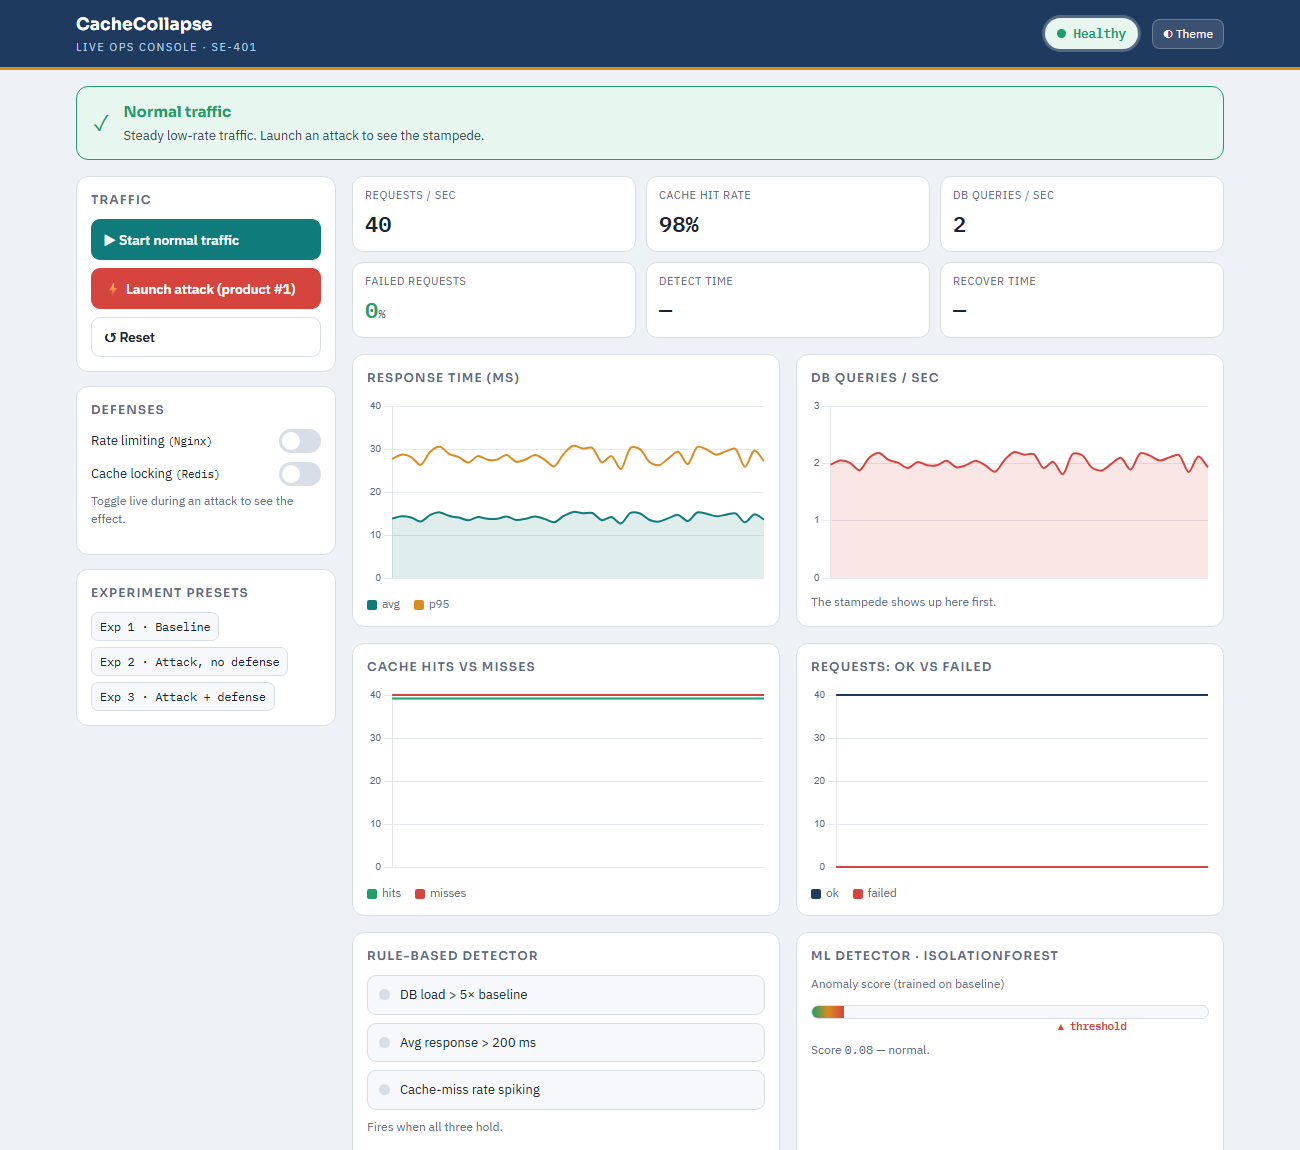
\includegraphics[width=\linewidth]{figures/ui-baseline.png}
\caption{Baseline}
\end{subfigure}\hfill
\begin{subfigure}[t]{0.32\linewidth}\centering
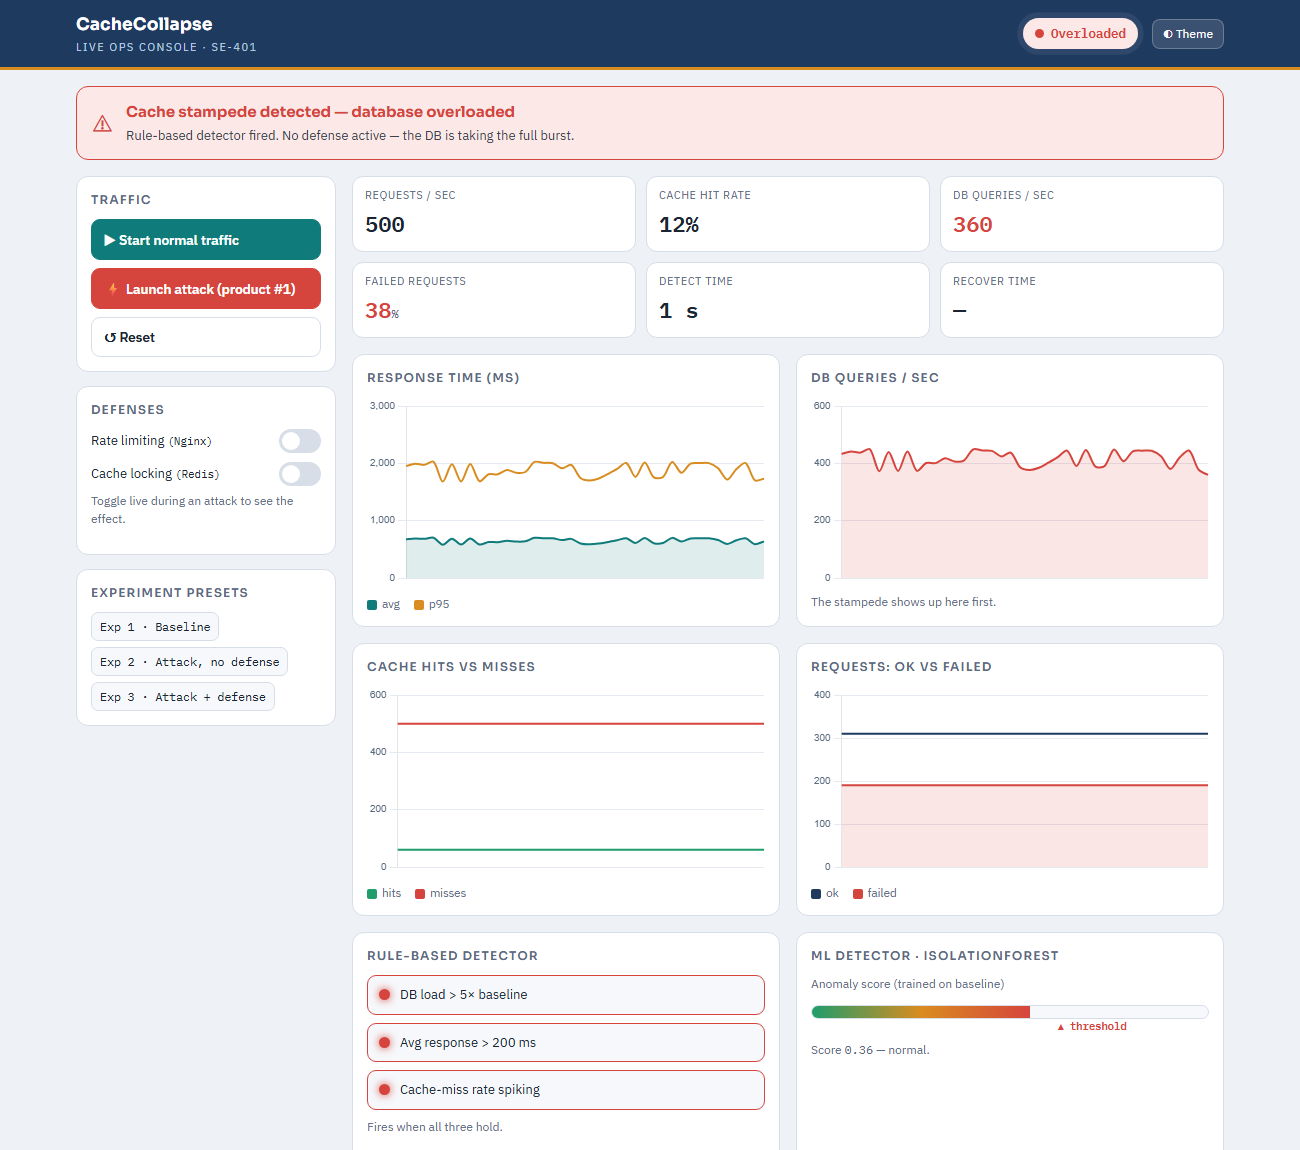
\includegraphics[width=\linewidth]{figures/ui-attack.png}
\caption{Attack, no defense}
\end{subfigure}\hfill
\begin{subfigure}[t]{0.32\linewidth}\centering
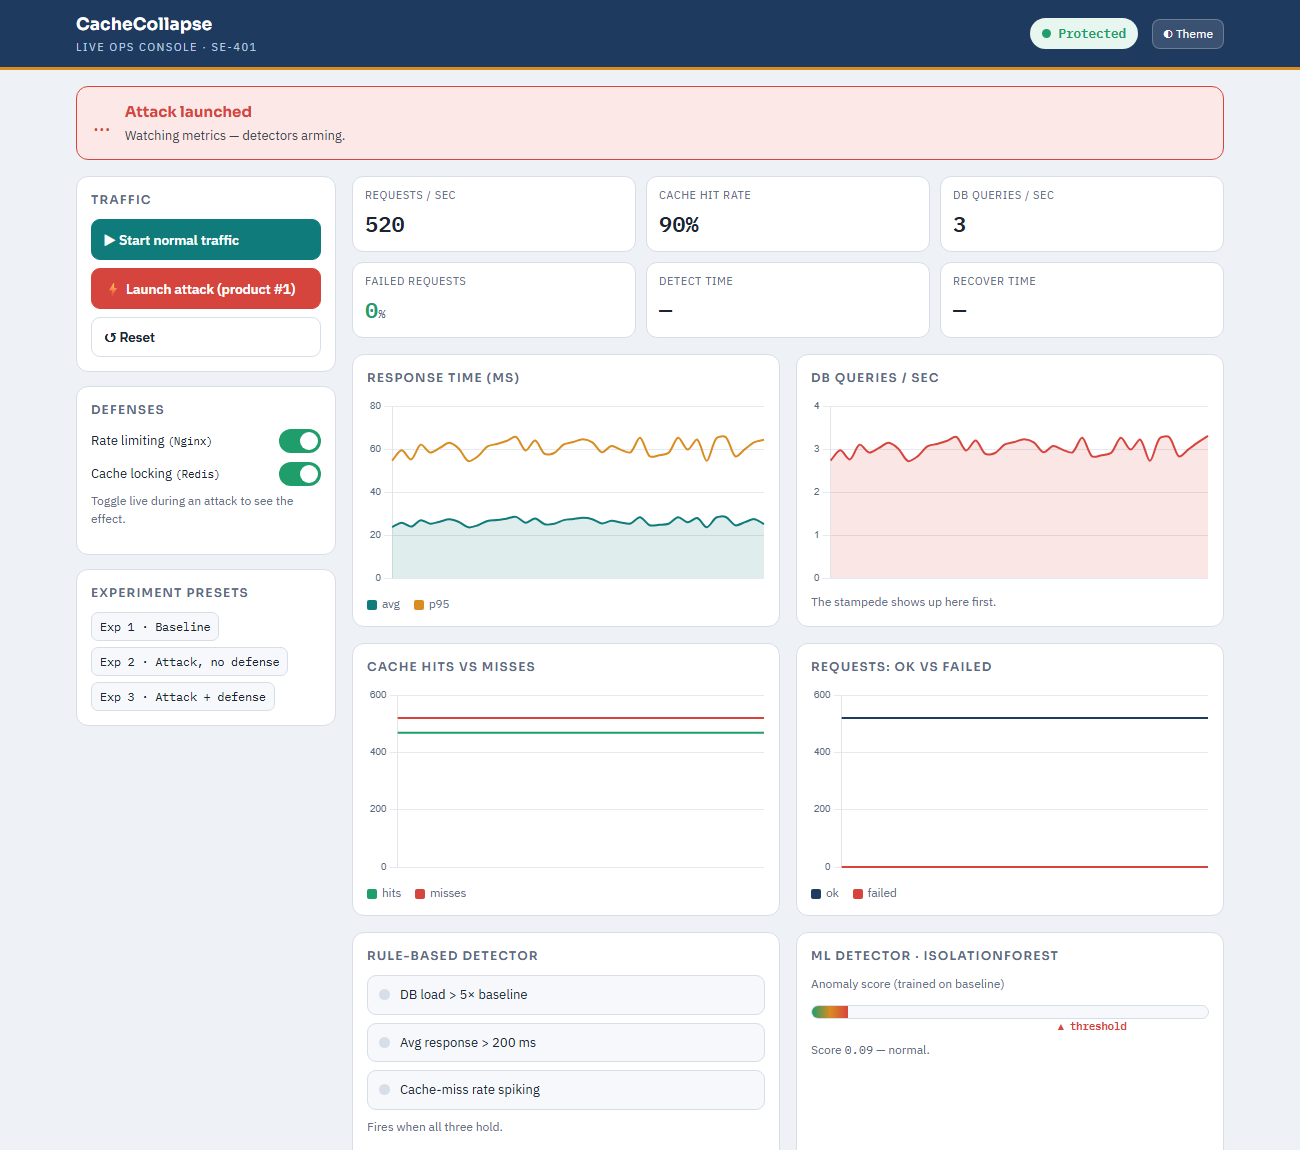
\includegraphics[width=\linewidth]{figures/ui-protected.png}
\caption{Attack with defenses}
\end{subfigure}
\caption{The live operations console in its three demonstration states. These are
\emph{design-phase mockup} screenshots driven by synthetic values to illustrate the
layout; they are not measurements. All quantitative results in this paper come from
the monitor's logs (Section~\ref{sec:results}).}
\label{fig:ui}
\end{figure}

\subsection{Configuration Parameters}
Table~\ref{tab:params} lists every tunable parameter and the value used in the final
configuration. Several values were changed during development (for example the TTL,
which the specification initially set to 10~s); the table reflects the code and
environment used for the results in Section~\ref{sec:results}.

\begin{table}[t]
\centering
\caption{Configuration parameters of the final configuration.}
\label{tab:params}
\small
\begin{tabularx}{\linewidth}{@{}L{4.4cm}L{2.2cm}Y@{}}
\toprule
Parameter & Value & Where / note \\
\midrule
Cache TTL $T$ & 4 s & \texttt{.env} \texttt{CACHE\_TTL}; short so stampedes recur \\
Stale TTL & $15T=60$ s (3{,}600 s pre-warm) & \texttt{app.py} \\
Simulated query time $d_0$ & 110 ms & \texttt{.env} \texttt{DB\_QUERY\_DELAY\_MS} \\
DB pool size $c$ (min) & 12 (2) & \texttt{db.py}; fail-fast \\
Lock expiry / loser poll / max wait & 3{,}000 / 50 / 1{,}500 ms & \texttt{app.py} \\
App rate limit $R$ & 50 req/s per client, 1 s window & \texttt{.env} \texttt{RATE\_LIMIT\_RPS} \\
Edge rate limit & 50 r/s, burst 20, \texttt{nodelay} & \texttt{nginx.conf} + dynamic include \\
Gunicorn (app) & 1 worker $\times$ 200 threads & \texttt{backend/Dockerfile} \\
Products $K$ & 100 & \texttt{seed.sql} \\
Normal traffic & 4 req/batch, 100 ms sleep ($\approx$18 req/s) & \texttt{loadgen.py} \\
Attack burst $B$ / hot pool $H$ / pause & 250 / 20 / 50 ms & \texttt{loadgen.py} \\
Monitor interval $\Delta$ & 0.5 s & \texttt{monitor/app.py} \\
Warm-up suppression $W$ & 6 intervals (3 s) & \texttt{monitor/app.py} \\
Rule: $K$, $\tau_L$, $\tau_m$, floor & 5, 200 ms, 0.5, 5 q/s & \texttt{detect\_rules.py} \\
Baseline EWMA weight & 0.2 & \texttt{monitor/app.py} \\
iForest: min train / window / contamination & 10 / 300 / 0.01 & \texttt{detect\_ml.py} \\
ML debounce & 2 consecutive intervals & \texttt{monitor/app.py} \\
Prometheus scrape interval & 2 s & \texttt{prometheus.yml} \\
\bottomrule
\end{tabularx}
\end{table}

\subsection{Reproducibility and Safe Operation}
The entire system starts with \texttt{docker compose up --build}; the database waits
for a \texttt{pg\_isready} health check before the application starts; and all
configuration is in version-controlled files plus a local \texttt{.env} that is
excluded from version control. The load generator targets only the stack's own proxy
on the private network, so attack traffic never leaves the host. The control endpoints
are deliberately unauthenticated for classroom demonstration; any deployment reachable
by others must restrict access, as discussed in Section~\ref{sec:ethics}. Appendix~A
gives a step-by-step reproduction guide.
